\documentclass[tikz,border=8mm]{standalone}
\usepackage[T1]{fontenc}
\definecolor{ink}{HTML}{243449}
\definecolor{muted}{HTML}{586575}
\definecolor{espresso}{HTML}{98502B}
\definecolor{milk}{HTML}{2866A6}
\definecolor{cold}{HTML}{008578}
\definecolor{sugar}{HTML}{9A3976}
\definecolor{decaf}{HTML}{6D61AC}
\begin{document}
\sffamily
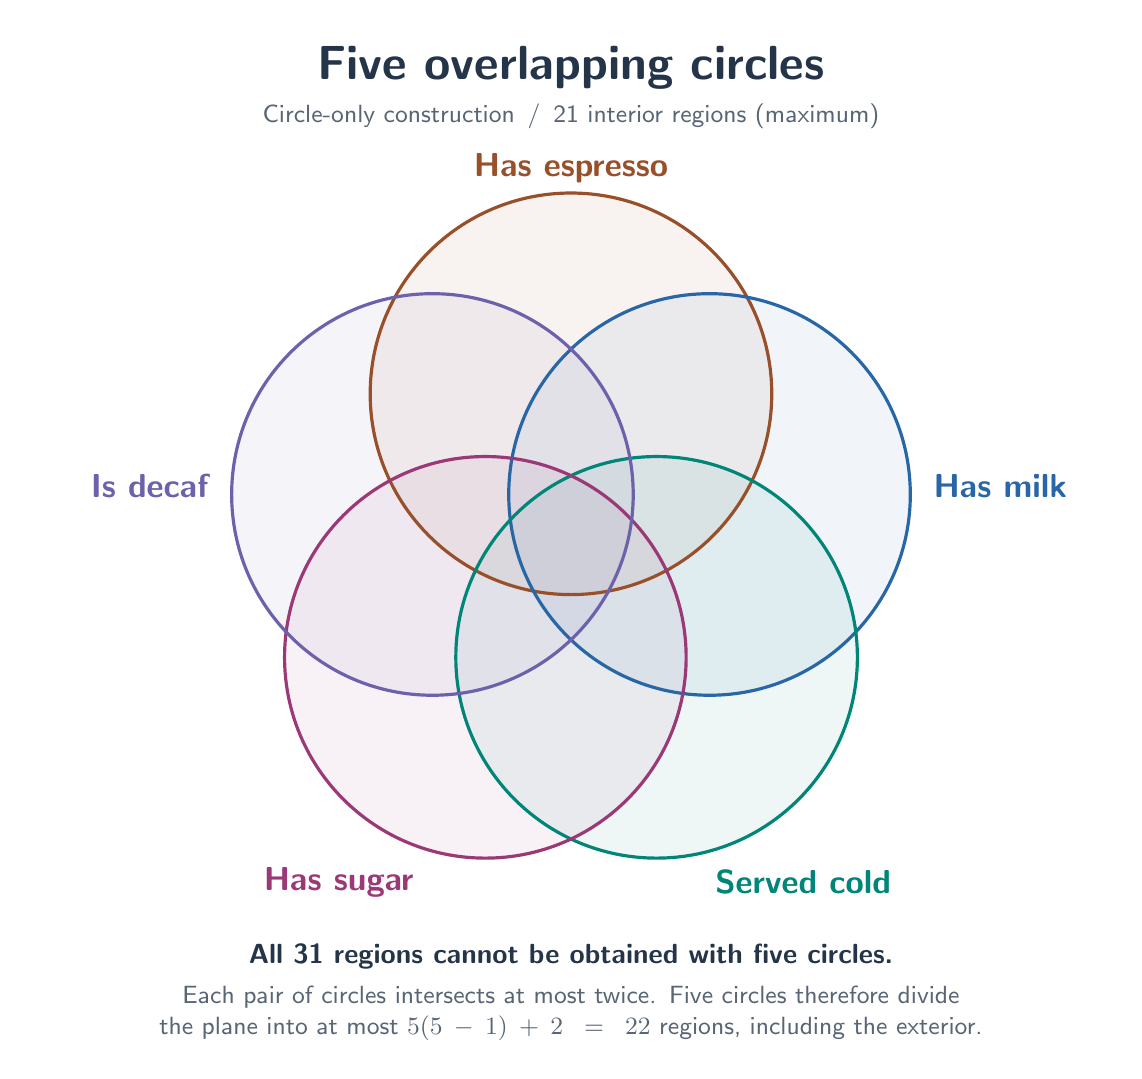
\begin{tikzpicture}[font=\sffamily, text=ink]
  \path[use as bounding box] (-6.9,-6.5) rectangle (6.9,6.5);
  \node[font=\sffamily\bfseries\LARGE] at (0,6.0) {Five overlapping circles};
  \node[font=\sffamily\small,text=muted] at (0,5.38)
    {Circle-only construction\enspace /\enspace 21 interior regions (maximum)};

  % In general position, n circles produce at most n(n-1)+2 faces.
  % Thus five circles can give 22 total faces, or 21 inside the union.
  % This regular pentagonal arrangement attains that bound, but is NOT
  % a five-set Venn diagram: ten of the 31 memberships are absent.
  \foreach \name/\angle in {A/90,B/18,C/-54,D/-126,E/162}
    {\coordinate (\name) at (\angle:1.85);}

  \foreach \name/\colour in {A/espresso,B/milk,C/cold,D/sugar,E/decaf}
    {\fill[\colour,opacity=0.065] (\name) circle[radius=2.55];}
  \foreach \name/\colour in {A/espresso,B/milk,C/cold,D/sugar,E/decaf}
    {\draw[\colour,line width=1.15pt] (\name) circle[radius=2.55];}

  \node[text=espresso,font=\sffamily\bfseries\large] at (0,4.72) {Has espresso};
  \node[text=milk,font=\sffamily\bfseries\large,anchor=west] at (4.48,0.68) {Has milk};
  \node[text=cold,font=\sffamily\bfseries\large] at (2.95,-4.35) {Served cold};
  \node[text=sugar,font=\sffamily\bfseries\large] at (-2.95,-4.35) {Has sugar};
  \node[text=decaf,font=\sffamily\bfseries\large,anchor=east] at (-4.48,0.68) {Is decaf};

  \node[font=\sffamily\bfseries\normalsize] at (0,-5.3)
    {All 31 regions cannot be obtained with five circles.};
  \node[text=muted,font=\sffamily\small,align=center,text width=13cm] at (0,-6.02)
    {Each pair of circles intersects at most twice. Five circles therefore divide\\
     the plane into at most $5(5-1)+2=22$ regions, including the exterior.};
\end{tikzpicture}
\end{document}
